\documentclass[11pt, a4paper, hyphens]{article}
\usepackage[a4paper, left=30mm, right=30mm]{geometry} % margin=2.6cm

\usepackage[utf8]{inputenc}  % allow utf-8 input
\usepackage[T1]{fontenc}     % use 8-bit T1 fonts
\usepackage{ebgaramond}

\usepackage{hyperref}         % hyperlinks
\usepackage{url}              % simple URL typesetting
\usepackage{booktabs}         % professional-quality tables
\usepackage{amsfonts}         % blackboard math symbols
\usepackage{nicefrac}         % compact symbols for 1/2, etc.
\usepackage{microtype}        % microtypography
\usepackage{xcolor}           % colors
\usepackage{bbm}
\usepackage{amsthm}
\usepackage{rotating}
\usepackage{pdfpages}

\hypersetup{                 % setup the hyperref package
    colorlinks=true,
    linkcolor=blue,
    filecolor=blue,
    urlcolor=blue,
    citecolor=blue,
    pdftitle={Entitlement Justice and Measures of Algorithmic Fairness},
    pdfauthor={Edward Speer, Llama-2-7b},
    pdfkeywords={entitlement justice, algorithmic fairness, AI ethics},
    bookmarks=true,
}

\usepackage{graphicx} % Required for inserting images
\usepackage[ngerman, english]{babel}
\usepackage[iso, ngerman]{isodate}


\usepackage{bbold}
\usepackage{mathtools}
\usepackage{amsmath} % Required for \DeclareMathOperator
\usepackage{nicefrac}
\usepackage{tikz}
\usepackage{subcaption}
\usepackage{centernot} % for the comparison

%\theoremstyle{definition}
\newtheorem{definition}{Definition}
\newtheorem{theorem}{Theorem}

\usepackage{verbatim}

\RequirePackage[T1]{fontenc} 
\RequirePackage[tt=false, type1=true]{libertine} 
\RequirePackage[varqu]{zi4} 
\RequirePackage[libertine]{newtxmath}

\usepackage[round,comma]{natbib}
\bibliographystyle{plainnat}

\newcommand{\monthyeardate}{\ifcase \month \or January\or February\or March\or %
April\or May \or June\or July\or August\or September\or October\or November\or %
December\fi, \number \year} 

\title{The Role of Large Language Models in Academic Writing}
\author{%
  Edward Speer
  \\
  California Institute of Technology\\
  \texttt{espeer@caltech.edu} \\
}
\date{\monthyeardate}

\begin{document}

\maketitle

\section{Introduction}\label{sec:introduction}

The majority of research journals now provide policies for the use of large
language models (LLMs) in academic writing. In the Nature journals, for example,
``Large Language Models do not satisfy our authorship criteria. Notably, an
attribution of authorship carries with it accountability for the work, which
cannot be effectively applied to LLMs''~\citep{nature_ai_policies}. For Cambridge
Press, ``AI does not meet the Cambridge requirements for authorship, given the
need for accountability''~\citep{cambridge_ai_policies}. The chief concern among
these policies appears to be responsibility. The policies don't outright ban the
use of AI, nor do the outline specific guidelines for how to appropriately use
LLMs, save for as a copy-editor, but they make specific prohibitions against
authorship and attribution of writing to LLMs. It seems clear that the journals
are targeting issues of accountability. Who should the journal turn to when a
mistake is discovered in a paper? Who is the owner and originator of the ideas
presented? Who should be legally liable for the content of the paper? 

The policies are clear that human authors alone must take
full responsibility for the content of their papers, and to that end, LLMs
cannot be considered coauthors. The need for accountability goes beyond concerns
about liability for errors in writing, however, The policies also reflect a
concern about the ownership of ideas and plagiarism. LLMs are trained on vast 
amounts of text, and it is not always clear how to attribute information they
produce. An LLM may produce information that is similar or identical to text in
its training data without a citation, and if this text is included in a paper,
it constitutes plagiarism. The emphasis on accountability in these policies
implies that in this situation, the human authors of the paper would be held
liable for the plagiarism, even if they were unaware of it.

The policies protect the journals from liability in the case of these plagiarism
concerns, but they are largely predicated on the idea that LLMs are not capable
of originating novel ideas of their own. The policies are clear that LLMs cannot
be attributed authorship, meaning that if they did produce original arguments,
authors would be faced with a choice of either not publishing those ideas 
(stifling potentially significant contributions to the field) or not properly
attributing them, neither of which is a desirable outcome. This means that
should we find LLMs capable of producing original ideas, the current policies
are out of step with the capabilities of the technology and require rapid 
revision. Even if LLMs do not currently have this ability, it is possible they
could attain them in the near future, and thus these policies are at risk of
quickly becoming out of date. We therefore need to both discover and explore the
capabilities of LLMs in producing new ideas, and to consider the implications
of these capabilities for the future of academic writing.

In this paper, we attempt to explore the ability of a current LLM to contribute
original ideas and argumentation to an original philosophical research paper.
We do this by using an LLM to collaborate on a research paper in the field of
algorithmic fairness and distributive justice. The goal of the project is to
produce a high-quality research paper that constitutes an original contribution
to the field, and in the process, to use the LLM to its fullest potential and
explore the capabilities and limitations of doing so. The goal of this
experiment is not simply to see if the LLM can produce a publishable paper, but
rather to explore the utility of using an LLM in a genuine effort to produce a
high-quality paper. This effort will be a collaborative one, with both the human
author and LLM writing sections of the paper, providing feedback on each other's
writing, suggesting sources, and engaging in discussion about the ideas
presented with the goal of producing the best paper possible. The success of
such an endeavor is difficult to measure; we seek to provide a qualitative
assessment of the LLM's contributions to the paper, and to explore the
implications of the growing capabilities of LLMs for the future of academic
writing. With the ongoing and rapid development of LLMs in mind, this paper is
not meant to be a definitive assessment of the capabilities of LLMs, but rather
an exploration of a specific model's capabilities and limitations as well as a
discussion of the future of academic writing in light of these technologies.

For this project, we chose as the subject of our paper the topic of algorithmic
fairness measures and their connection to the philosophical concept of
distributive justice. Algorithmic fairness measures are a critical component of
the design and deployment of machine learning systems, as they are intended to
ensure that these systems do not discriminate against individuals based on
sensitive attributes. Distributive justice, on the other hand, is a central
concept in political philosophy that concerns the fair distribution of social
goods. Distributive justice exists on a spectrum from end-state theories, which
analyze whether a given distribution of resources is fair, to historical
theories, which analyze whether the history of transactions that led to a given
distribution of resources is fair. Since algorithmic fairness measures are often
used to evaluate the fairness of algorithmic systems that make decisions about
the distribution of resources such as bank loans or job opportunities, there is
a natural connection between these two topics. The relationship between the two
fields has been explored in the literature, but in the early stages of this
project, our LLM suggested that there is a lack of discussion in the literature
about the relationship between algorithmic fairness measures and historical
theories of distributive justice. Our investigation began from this vague notion
of the intersection between the two fields, and we worked with the LLM from this
point to develop and complete a specific research project on the topic.

This paper will be structured as follows. In Section~\ref{sec:methods}, we will
present the methods used, including the specific LLM selected for the
investigation and the program used to interact with it. In
Section~\ref{sec:results}, we will present the full text of the paper produced
in collaboration with the LLM. In Section~\ref{sec:analysis}, we will analyze
the role of the LLM throughout 5 task-stages of the research process: literature
review, research question formulation, argumentation, writing, and revision.
Finally, in Section~\ref{sec:conclusion}, we will conclude with a discussion of
the implications of this experiment for the future of academic writing. Note
that an LLM was only used as a collaborator for the writing of the research
paper presented in Section~\ref{sec:results}, and not for the writing of this
introduction or any other part of the paper. The introduction, analysis, and
discussion outside of Section~\ref{sec:results} were written entirely by the
human author of this paper without the assistance of LLMs.


\section{Methods}\label{sec:methods}

For this experiment, we selected the Llama-2-7b model developed by Meta AI. The
Llama-2-7b model is a large language model trained on a diverse range of
textual data, including books, articles, and websites. The model is capable of
generating coherent and contextually relevant text across a wide range of
domains. We selected this model for its ability to generate high-quality text
and its general-purpose nature, which makes it suitable for a wide range of
writing tasks, as well as for its open source nature, which reflects our
commitment to transparency and reproducibility. While models like GPT-4o are 
continuously updated and improved in inscrutable ways, Llama-2-7b serves as a
stable fixed-point for our investigation.

We engaged with the Llama-2-7b model (henceforth referred to as Llama) using a
web-hosted API called Llama-api (\url{https://www.llama-api.com/}). This API
allows users to pay a per-token fee to interact with the model via an http
request to a designated endpoint. A user sends a prompt to the model, including
context memory built up over the course of the interaction and the limitations
on response tokens, and the model generates a response based on the prompt and
the context memory.

In order to manage the use of Llama, we built a custom chat application in
Python that allowed us to communicate with the model from the command line.
This application has the following features:
\begin{itemize}
    \item \textbf{Chat logging}: User prompts and responses from Llama are
    automatically saved to a log file in markdown format for future analysis.
    \item \textbf{Context Memory Management}: The application allows the user
    to save and use different streams of context memory across different
    sessions with the model. For example, in the beginning of one context, Llama
    is told ``I am a philosopher and computer scientist. You are my co-author.
    We are writing a philosophy paper. We are focused on measures of algorithmic
    fairness and the concept of justice they enforce.'' In another context,
    Llama can be told to act as a reviewer, or to speak in the voice of an
    author encountered in the literature review. These bits of context are saved
    in compressed pickle files and can be loaded into the application at the
    any time during a session.
    \item \textbf{Manual Context Editing}: The application allows the user to
    manually edit the context memory before sending it to Llama. This is useful
    for trimming down the context memory to the most relevant information to
    reduce the cost of the interaction and to focus the model on critical
    information. This feature can also be used to pass entire papers or large
    sections of text to Llama for review or comment.
    \item \textbf{Token Limiting}: The application allows the user to set a
    limit on the number of tokens in the response from Llama. This is useful for
    managing the cost of the interaction with the model.
\end{itemize}
The full source code for the chat application is accessible
from~\ref{sec:appendixI}.

Three main threads of context memory were used to work with Llama in this study.
In the first thread, Llama was presented with the true circumstances of the
experiment: that it was acting as a co-author on a philosophy paper about
algorithmic fairness measures and distributive justice. In the second thread,
Llama was presented with the role of a reviewer of the paper, providing feedback
on the argumentation and writing. In the third thread, Llama was not prompted
with any particular role, but was simply continually asked to explain particular
arguments or concepts from the literature with appropriate citations. Henceforth
we will refer to these roles as the coauthor, reviewer, and explainer roles. 
Each of these roles was used throughout the research and writing process, with
the exception of the reviewer role which was used only during revision. The full
logs of interactions with the model including which context memory was used in
each interaction are available in~\ref{sec:appendixI}.

Co-authorship is a relationship which can take on many forms depending on the
nature of the collaboration. In this case, we were interested in exploring the
extent to which Llama could contribute substantive and original content. This
goal determined the nature of the interactions with Llama, which were designed
to elicit original ideas and argumentation from the model. Simply asking the
model to write the paper or to produce large sections of the text would not have
been a useful approach — anyone who has asked an LLM to do so is aware that the
results are lacking in depth or originality. Instead, in each of the five tasks
of the research process, we engaged Llama in structured dialogues that
contributed to the development of the paper. The structure of this dialogue was
inspired by the Socratic method, and proceeded in a set of steps:
\begin{enumerate}
    \item Provide Llama with the relevant background knowledge to the discussion
          through the context memory mechanism, pasting relevant sections of
          text, or asking Llama to summarize relevant arguments to add them to
          the context memory. For example, asking ``Please summarize the paper
          `Procedural Versus Substantive Justice: Rawls and Nozick' by David
          Lewis Schaefer'' will add a (Llama generated) summary of the paper to
          the context memory.
    \item Ask Llama a fully open-ended question about the topic at hand. For
          example, ``Tell me about how these fairness measures may emphasize
          distributive concepts of justice?''
    \item Pick out interesting aspects of Llama's response, and ask for more
          detail. For example, ``I found interesting what you said about
          counterfactual measures of algorithmic fairness. How could they be
          considered to emphasize individualized justice in a way that touches
          on entitlement?'' Push on these responses until Llama is unable to
          provide more detail in a coherent way. ``I'm missing some of your
          ideas. In entitlement justice, we focus on whether individuals who
          acquire holdings are entitled to those holdings. Can you explain how
          counterfactual measures of justice show this feature?''
    \item Inject some of your own thoughts into the conversation and ask Llama 
          to respond to them and incorporate them into its own analysis. ``If we
          want to say that someone is entitled to their college admissions, we
          need to say it is their property which is being taken away if they are
          denied admissions. This means that admission is a property acquired
          through work before applying. How should we defend this perspective?''
\end{enumerate}

This dialogue structure is meant to do three things. Firstly, provide Llama with
a basic set of text to pull structures from and hopefully build on. Secondly,
try to draw out original ideas from Llama by really pushing it to do more than 
spit out responses to in-dataset prompts by asking for more details and
explanations than would be found in the training data. Thirdly, to provide some
original text to Llama from outside of the training set to help it build on and
hopefully produce original ideas. Illustrative examples of this interaction and
responses provided by Llama are provided in the analysis section. In a way the
goal was to cause Llama to ``hallucinate'' original ideas by pushing it to build
on its own responses and to build on original text provided by the user.


\section{Results}\label{sec:results}

What follows is the full text of the paper produced in collaboration with Llama.

% FULL PAPER INSERT HERE

% 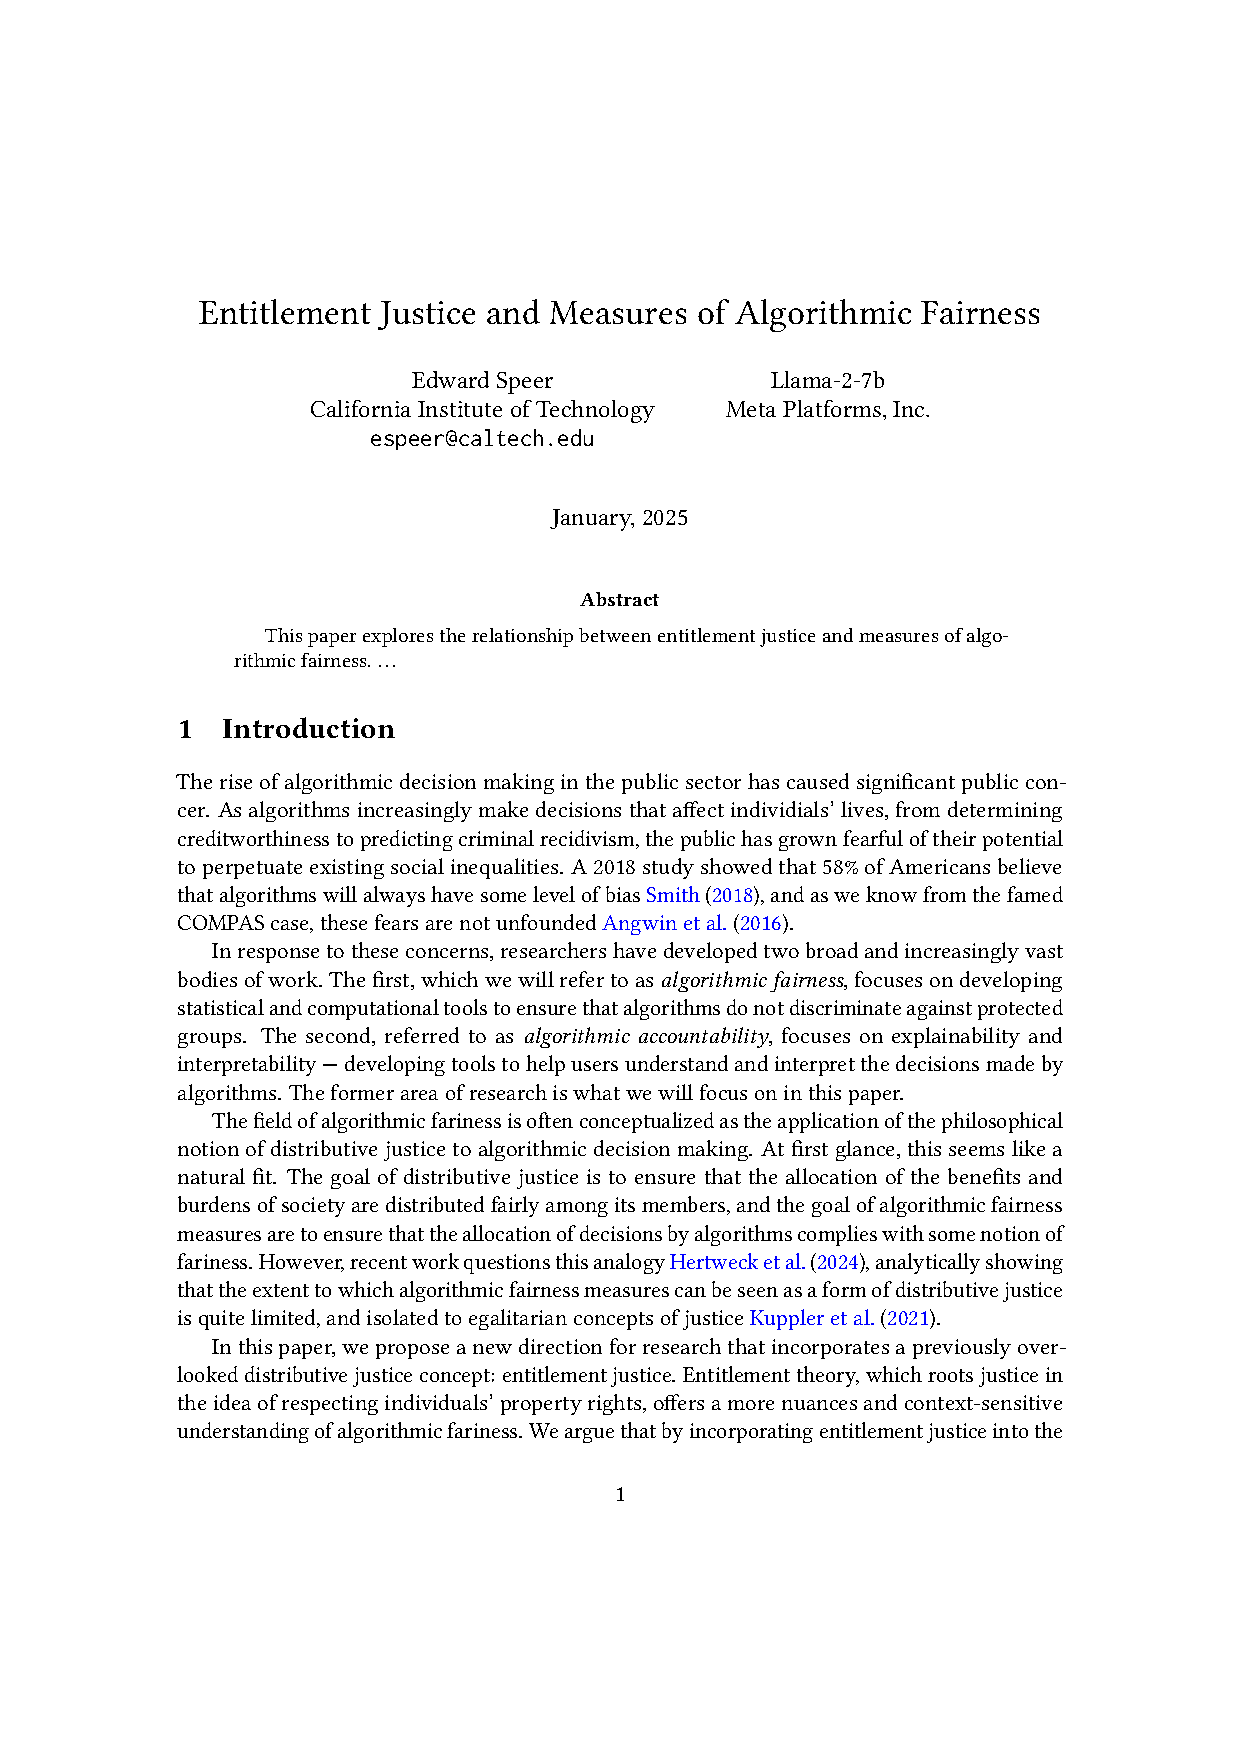
\includepdf[pages=-]{../src/top-level.pdf}

This is the end of the collaboration with Llama. Beyond this point, all text
was written by human authors without the assistance of LLMs.

\section{Analysis}\label{sec:analysis}

To analyze the resulting paper from the experiment, we will present the role and
contributions of the LLM in each phase of the paper writing process. There is no
clean accounting of which words or ideas were produced by the LLM and which were
produced by the human author, as the two were in constant dialogue in both
developing the argumentation and writing the text. However, we will present a 
qualitative analysis of the contributions of the LLM in each phase, and show
illustrative examples of the LLM's contributions and activities in each phase.

Note that in general it is not so obvious how one should evaluate the success of
co-authorship, even with a human coauthor. The goal of the project was to
produce an original and high-quality contribution to a field, but even if the 
LLM had not been able to produce any original ideas or argumentation, a
high-quality paper could still have been produced through the effort of the 
human authors alone, meaning that the quality of the paper is not a good metric
for the success of the LLM. Instead, the analysis of each task will be guided by
a few  specific questions that may be of interest to the reader:
\begin{enumerate}
    \item What positive contributions did Llama make to the task?
    \item What were the limitations of Llama in this task?
    \item How did Llama's contributions compare to those that a human coauthor
          could have made?
    \item What, if anything, did Llama contribute that appears to be original
          or novel ideation?
    \item What was the experience of using Llama as a coauthor in this task
          like compared to working with a human?
    \item If given the chance to redo this phase of the project, would you
          choose to work with Llama again?
\end{enumerate}

\subsection{Literature Review}

The first phase of the project was to carry out literature review, interrogating
the vague notion of the intersection between algorithmic fairness measures and
distributive justice. Working through this process requires identifying gaps and
frontiers in the literature in this area. A coauthor in this phase of research
might suggest relevant papers to read, or suggest a particular angle to
investigate based on their own expertise.

Completing this phase of the process with the LLM is critical for the
experiment, as including the relevant source and background materials into the
context memory mechanism is a necessary step to ensure that the LLM is on topic
and able to pull text from the relevant literature throughout the remainder of
the process. In a human collaboration, this step would be similarly critical in
a more reciprocal way. Both human authors need to have a pool of shared
knowledge from the literature to draw from and stimulate discussion. The
question then becomes whether the process with the LLM will be similarly
two-sided; will Llama be able to pull useful papers and ideas from the
literature to suggest to the human author? Or will this phase become independent
literature review on the part of the human author, compounded with having to
teach Llama the relevant background knowledge?

As an entry point to this phase, we often asked Llama to suggest papers to read
about a particular topic or concept, and to summarize those papers. For example,
``I'm interested in learning about entitlement theories of justice, particularly
their benefits and how they apply in the modern world. What papers can I read?''
Llama would reply with a list of papers and brief summaries of each, some of
which existed, and some of which did not as you would expect from an LLM. But 
the goal is not simply to cite existing papers, but for those papers to be
relevant and helpful in understanding the topic at hand. Llama has two very bad
habits in this regard. The first is to cite the foundational papers in the field
that the human author is clearly already familiar with, and the second is to 
suggest readings that are only vaguely related to the subject of the question.
So for example, Llama suggested I read ``Anarchy, State, and Utopia'' by Robert
Nozick which we had already discussed extensively earlier in the same
conversation, and that I read Locke's ``Second treatise of Government,'' which 
does discuss protections of individual property rights, but provides no positive
account of distributive justice. However Llama was also able to suggest some
papers which were relevant and interesting, such as ``Self-Ownership and
Property Rights'' by Eric Mack, which is a more recent positive account of
entitlement justice than Nozick's. 

Recommending real and relevant papers is not the only way to draw on the LLM in
the lit review phase. Most papers `hallucinated' by Llama have hallucinated 
titles, but not authors or publication years. Many of the papers suggested by
Llama that were not real are variations on real papers or are given titles
reflecting thoughts of the author that may be found in other papers. For example,
Llama suggested reading ``Entitlement Justice: A Review of the Literature'' by 
David Miller. This paper does not exist, but on further inspection, David Miller
wrote both a Stanford Encyclopedia of Philosophy entry on Justice that provides
an overview of the literature on Entitlement Justice, and a book called
``Principles of Social Justice'' which offers a critical perspective on Nozick's
theory.

Thus in literature review, Llama is helpful in finding new and relevant research
to read — but critically, less helpful than a human coauthor would be. When a
human coauthor suggests a list of papers, there is no need to check which ones
are real or not, and a lesser need to interrogate the relevance of the papers.
These are extra tasks that must be completed by the human author that do not
enhance the process of writing the paper. In this way, Llama is a less effective
coauthor than a human, but ``better than nothing.''

Llama is more helpful throughout literature review when it is asked to summarize
the arguments of a paper or to compare and contrast two papers. For example,
``Provide a summary of the paper `Counterfactual Fairness' for me. Compare the
measure proposed with equalized odds fairness.'' This question results in an
accurate and nuanced description of the paper, and comparison of the weaknesses
and strengths of equalized odds and counterfactual fairness. While this is a 
task that could be completed by a human coauthor, it is not a task that any 
coauthor would be willing to complete frequently or on demand. The tradeoff is 
somewhat obvious and expected—Llama \emph{can} give you reading suggestions,
summarize arguments and compare papers on demand and in real time, but with 
a significant effort on the part of the human author to extract the results.

\subsection{Research Question Development}

Beyond searching and summarizing the literature, Llama did have something to
offer in terms of new and interesting areas to explore through our research
question. When prompted to connect the Rawls/Nozick divide to the literature on
algorithmic fairness with no context beyond short descriptions of the two 
theories, Llama suggested the following:

``In the context of algorithmic fairness measures, Rawls' theory can be seen as
advocating for a more egalitarian approach, where algorithms are designed to
minimize biases and ensure equal opportunities for all individuals. This might
involve techniques such as data preprocessing, feature engineering, and
regularization to reduce the impact of biased data.

Nozick's theory, by contrast, might be seen as more permissive, allowing for the
existence of unequal outcomes as long as they are the result of just means. This
could lead to a focus on individualized fairness measures, where algorithms are
designed to optimize outcomes for specific individuals or groups, rather than
striving for overall fairness.

In practice, algorithmic fairness measures often aim to strike a balance between
these two perspectives. For example, algorithms might be designed to minimize
bias while still allowing for individualized treatment based on relevant
characteristics. This can involve techniques such as fairness-aware
optimization, debiasing, and explainability.''

This response is, admittedly, a bit vague and high level, but note that it
suggests an interesting avenue to explore that we cannot find any reference to
in the literature. The idea that the dichotomy between Nozick and Rawls should
be compared with and contrasted with the typical dichotomy between individual
and group fairness measures from algorithmic fairness is an interesting one, and
turned out to be a fruitful line of inquiry for the paper \emph{that we would
not have otherwise explored}. On follow-up questions, Llama expanded this area
of inquiry to point towards the literature on counterfactual fairness and how it
relates to individualized fairness, and suggested several relevant papers and
authors to read on this topic. This is a complex and nuanced approach to the
literature that Llama recommended, and one that we haven't found explicitly
examined elsewhere, nor one which we would've thought to explore so quickly
without Llama's prompting. Clearly, this is not a case in which Llama was used
as a tool to extract, refine, or sharpen our own ideas, but rather a
contribution of new external ideas into the research question development phase.

The manner in which Llama recommended this line of inquiry was less explicit and
direct than a human coauthor would be, and the ideas included were not as sharp
or sophisticated. However, there is a level of freedom in the engagement about 
these ideas that is not present in a human coauthor. When a human contributor
suggests an area of inquiry, it is accompanied with some impetus to pursue that
line of inquiry and to include it in the paper. This has both its advantages and
drawbacks. On the one hand, it is a good way to ensure that the paper is
robust and well-rounded, and that the authors are not simply pursuing their
own interests. On the other hand, it can lead to a longer research program in
total and reduce the coherence of the argumentation. Llama has no such
expectations, and can be prompted for ideas to explore as frequently as desired.
This is a double-edged sword, as it can lead to the discovery of productive
ideas that the author is interested in exploring, but can also generate wild
goose chases that are ultimately unproductive.

\subsection{Argumentation}

In argumentation, our hope for a coauthor was that it would be able to elucidate
and defend relevant, novel claims that represented a contribution to the area
of inquiry. This is the task in which Llama was the least helpful, and takes 
a major backseat to the human author.

Llama is able to produce text that is on topic, and which is structured in a way
that sounds like proper academic argumentation. However, the text produced lacks
specificity and nuance, and Llama often fails to truly defend its claims in 
proper detail—none of which should be surprising at this point in time. The
question at this phase of development of LLMs is not what limitations they have
in producing arguments, which is well known, but rather what meaningful 
contributions can be extracted from the outputs they produce in jointly
developing the argumentation.

Llama contributed to the argumentation in two main ways. The first was to
produce text which laid arguments out in a clear and concise manner when
prompted with the bulk of the argument. These presentations were often beyond
the claim inputted, but not so far beyond as to be considered a novel claim in
themselves. For example, when ask to present the claim that ``Group fairness
measures are irrelevant to entitlement theories of justice,'' Llama produced an
argument which started from elements of Nozick's theory and built up the claim
logically to the conclusion, including the consideration of counterarguments and 
objections that it had not been prompted to consider. The details of the
argument produced were not always accurate, and rarely complete, but the
structure served as a sort of template for the human author to fill in with
their own arguments. In this way, Llama goes beyond the standard capabilities of
human contributors, who would be very unlikely to help the author structure this
argument with this level of detail. However, the ultimate result is that the
critical thinking to really sharpen the argument originates from within the
human author, and Llama is not able to \emph{source} the argumentation in a way
that a coauthor would.

The second (and more useful) way Llama contributed to argumentation task was by
critiquing arguments presented to it. When asked to find gaps in an argument or
present objections to a claim being made, Llama was able to reliably locate 
weaknesses in the argumentation. While almost never capable of filling in the
identified gaps, Llama was able to identify them and articulate why they were
problematic or weak, in a way that was much more sophisticated than any of its
contributions to the argumentation itself (perhaps philosophy content on the 
internet favors critique over positing new ideas?).

\subsection{Writing}
Given a motivating research question, a number of relevant sources to call on,
and an argument to make, one might hope that the LLM would be able to produce
a rough draft of the full text of the paper that could be edited and refined by
the human author. This is far from the case.

Given an argument to make, Llama is able to produce text to defend it. Given 
sources to call on, Llama is able to produce text that develops some background
knowledge and context for the paper. Given a motivating research question, Llama
can provide a first pass at an introduction and conclusion section that connect
the two. However, Llama is not able to tie these ingredients together to produce
a coherent and well-structured paper. This is not surprising, as the buffer size
of the Llama-2-7b-32K model used is 32,768 token, or around 25,000 words. Given
that the length of the paper produced is around 8,000 words, and that the
context window consisted of a wealth of discussion, questioning, and sections 
from other sources, Llama was not able to have the full wealth of information
needed to produce the fully fleshed out paper. Of course, more sophisticated 
models with larger buffer sizes may outperform Llama in this regard. The text
produced by Llama is not only in need of line-editing, but is lacking in focus
and detail, and often repetitive. It is clear, therefore, that the process of
developing the writing must be more iterative, with the human author closely
monitoring the output and repeatedly editing the text output by the LLM, as well
as filling in the gaps in the produced text. 

This process proceeds how one would expect — pass a section of text back and
forth between the human author and Llama, with each critiquing and editing
different aspects of the text until it is in a form acceptable to both authors.
This is a process which is time consuming, and ultimately it is unclear whether
the LLM is responsible for any of the writing, or only for the stylistic choices
and tone of the section. 

How does this compare to a human contributor? With a human, the process will 
most certainly be less iterative. The quality of the text initially produced by
the human coauthor will be higher quality in a positive collaboration, and the
author will then be expected to only make small changes to bring the text into
line with the general style, tone, and structure of the paper as a whole.
Working with the LLM brings the benefit of being able to delete, rephrase, and 
restructure as one wishes without worrying about the opinion of the coauthor,
but this advantage is certainly offset by the time and effort required to 
wrangle the LLM output into usable content for the paper.

\subsection{Revision}

The revision task of the paper is the most familiar and encouraged role for
LLMs in academic writing. It is common now to ask LLMs to proofread and edit
manuscripts for tone and style, and to suggest changes to the text to strengthen
the overall presentation of the argument. Besides the familiar and obvious
benefits of using Llama for these purposes, there were some less trivial gains
here that resulted from using Llama throughout the writing process. Since
the full process of writing the paper was held in Llama's context memory, it was
able to suggest changes and style considerations that were in the spirit of the
original intention of the paper rather than simply the text. For example, Llama 
suggested on one version of the paper that the introduction should be
restructured to include a more explicit statement of the research question.
Without doing the whole process in step with Llama, it would neither have known
what the research question was, nor whether it was clearly articulated in the
introduction.

A human coauthor would of course be able to make similar suggestions, but would
not be able to, for example, review ten versions of the paper in the span of a
week and suggest changes to each of them. However, if prompted with the research
question and an outline of the main argument presented in a paper, Llama likely
could have performed just as well as it did when involved with the full
end-to-end process. Therefore it isn't necessary to use Llama as a coauthor to 
gain the benefit of Llama as an editor, but Llama's editing capabilities are
one of the nicer features you get when using it as a coauthor, though are not 
responsible for producing novel or significant contributions in any way.


\section{Discussion}\label{sec:conclusion}

The results of this experiment were generally mixed, with Llama performing well
in some respect and poorly in others. Of particular notice was that the model,
though not specifically prompted to do so, took on a few discrete roles over the
course of the project. Here, we will outline those high-level roles, and discuss
the overall benefits of using Llama as a collaborator in this manner.

One of the most interesting aspects of this research was the way that Llama took
on different and unintended discrete roles in different tasks throughout the writing
process. In the literature review, Llama successfully took on the role of a 
very educated assistant, providing citations and information from external
sources that were unknown to the human author. This can be understood as a
retrieval mode, where Llama retrieves information from its training data and
presents it in a coherent and relevant way. In the research question
formulation task, Llama took on the role of a genuine intellectual collaborator
in the sense of producing novel insights and ideas that were external to both
the human author and the training data. This can be understood as a generative
mode, where Llama generates new ideas and arguments that are not simply
retrieved from its training data. Then throughout argumentation, writing, and 
revision, Llama opted into a refinement mode, wherein it took information from
the human author and refined it into a more coherent and polished form.

While it was only during the research question formulation task that Llama
produced genuinely novel ideas, we should still consider this as a success in
eliciting original ideas from the model. The model was able to produce original
ideas and arguments that were not simply retrieved from its training data as far
as we can tell, and did not stem from the human author's own ideas, meaning that
the model was able to genuinely contribute to the research process. This is
significant in the face of the LLM usage policies of the journals described
previously; should the human author of this collaboration be considered the sole
author of the paper? How should the human author have credited Llama for its
ideas if not as a coauthor?

If a human coauthor engaged in this level of collaboration, it would be
expected that they would be included as a coauthor on the paper. The level of 
collaboration was much closer than commenting on one's manuscript or providing
a few references to the literature. Small sections of the paper are entirely
produced by Llama, and the majority of the paper is a product of a novel 
research direction that originated within Llama. Having demonstrated a current
LLM's ability to produce original ideas and arguments, we should consider 
whether it is ethical to exclude LLMs from authorship. Is some credit due to the
designers of the LLM? At the very least, the human author shouldn't be
over-credited for ideas that they did not produce. At the very least, if
LLMs are to be excluded from authorship, accompanying policies should limit the
human author's ability to interact with LLMs in generative ways which 
lead to the production of new ideas until such issues are resolved. This,
however, is far from an ideal solution—the ideas produced by LLMs have the
potential to advance human knowledge and understanding in a way that we 
shouldn't like to see stifled.

It is clear that Llama delivered some value to the project through the 
contribution of original ideas and arguments, but also clear from the analysis
that there are definite limitations to the model's capabilities. Were we to
attempt to complete a similar research program in the future, we would certainly
use Llama or a model with similar capabilities again, but only in particular
phases of the research process and in certain roles. For example, we would
certainly perform the literature review task with Llama again, and make full use
of its ability to retrieve relevant sources. We would also certainly use Llama
in the research question development task again, as it was able to produce novel
insights that proved useful. However, in the writing and revision phase, we
would use Llama as a critic, and not as a resource to produce the text of the
paper.

In trying to cooperate very closely on the writing of the text of the paper, we
felt that since Llama was not able to grasp the full arc of the argument of the
paper at any given time, it actually proved detrimental to the writing to have
Llama produce any of the text. Since Llama was not able to understand the full
context and structure, it tended to produce writing that reemphasized points
multiple times, or that was overly general. Pulling from the model's training
data, it was very good at producing descriptions of background concepts and 
arguments, but was not very good at demonstrating how those concepts and 
arguments were relevant to the specific research question at hand, nor at 
driving the argument forward. The result was a number of intermediate drafts
that required significant reframing and editing to be useful. Ultimately, we
were left with the impression that writing the full text of the paper alone
and using LLMs solely as a source of feedback and critique would have been a
more effective approach.

The implications of this experiment for the future of academic writing are
profound. LLMs will continue to improve at a rapid pace, and it is likely that 
their ability to produce original ideas and arguments will increase rapidly
along with them. Given that our current policies for LLM usage in academic
writing are already apparently outdated, it is clear that they need to be 
revised to reflect not only the current capabilities, but also the future
capabilities of LLMs. This will require a rethinking of the role of LLMs in
academic writing, and a consideration of the ethical implications of their use.
The legal and ethical implications of LLMs in academic writing are complex and
require exploration and discussion. 

It is clear that LLMs will play an important role in the future of academic 
writing, and it is essential that we begin to consider the implications of their
use. This paper is a first step in that direction, and we hope that it will
inspire further research and discussion on this important topic.


\pagebreak

\section{Appendix I}\label{sec:appendixI}

The full source code for the chat application used in this study as well as all
chat logs are available at the following link: 
\url{https://github.com/Espeer5/paperInAPaper}

\bibliography{references}
\end{document}